\documentclass{beamer}

\usepackage[utf8]{inputenc}
\usepackage{beamerthemesplit}
\usepackage{url}
\usepackage{hyperref}
\usepackage{tikz}
\usepackage{alltt}

\usepackage{listings}
\usepackage{marvosym}
\usepackage{color}
\usepackage[multidot]{grffile}
\usepackage{multirow}
\usepackage{array}
\usepackage{setspace}

\usepackage{CJKutf8}
\newcommand{\zhs}[1]{\begin{CJK}{UTF8}{gbsn}#1\end{CJK}}

\usetheme{Madrid}

\usecolortheme[RGB={132,186,75}]{structure}
\definecolor{cactusgreen}{RGB}{132,186,75}
\newcommand{\red}[1]{\textcolor{cactusgreen}{#1}}
\newcommand{\black}[1]{\textcolor{black}{#1}}

\graphicspath{{../pics/}}

\logo{
\includegraphics[height=0.7cm]{CLR_HOR}} 

\newcommand{\head}[2]
 {\frame{\frametitle{}\begin{centering}\LARGE#1\\#2\end{centering}}}

\newcommand{\abspic}[4]
 {\vspace{ #2\paperheight}\hspace{ #3\paperwidth}\includegraphics[height=#4\paperheight]{#1}\\
  \vspace{-#2\paperheight}\vspace{-#4\paperheight}\vspace{-0.0038\paperheight}}

\newcommand{\picw}[4]{{
 \usebackgroundtemplate{
 \color{black}\vrule width\paperwidth height\paperheight\hspace{-\paperwidth}\hspace{-0.01\paperwidth}
 \hspace{#4\paperwidth}\includegraphics[width=#3\paperwidth, height=\paperheight]{#1}}\logo{}
 \frame[plain]{\frametitle{#2}}
}}
\newcommand{\pic}[2]{\picw{#1}{#2}{}{0}}

\newcommand{\question}[1]{\frame{\begin{centering}\Huge #1\\\end{centering}}}
\newcommand{\redidot}{\makebox[0mm]{\hphantom{i}\red{i}}{\i}}
\newcommand{\blackidot}{\makebox[0mm]{\hphantom{i}\black{i}}{\i}}

% We want to use the infolines outer theme because it uses so less space, but
% it also tries to print an institution and the slide numbers
% Therefore, we here redefine the footline ourselfes - mostly a copy & paste from
% /usr/share/texmf/tex/latex/beamer/themes/outer/beamerouterthemeinfolines.sty
\defbeamertemplate*{footline}{infolines theme without institution and slide numbers}
{
  \leavevmode%
  \hbox{%
  \begin{beamercolorbox}[wd=.25\paperwidth,ht=2.25ex,dp=1ex,center]{author in head/foot}%
    \usebeamerfont{author in head/foot}\insertshortauthor
  \end{beamercolorbox}%
  \begin{beamercolorbox}[wd=.5\paperwidth,ht=2.25ex,dp=1ex,center]{title in head/foot}%
    \usebeamerfont{title in head/foot}\insertshorttitle
  \end{beamercolorbox}%
  \begin{beamercolorbox}[wd=.25\paperwidth,ht=2.25ex,dp=1ex,center]{date in head/foot}%
    \usebeamerfont{date in head/foot}\insertshortdate{}
  \end{beamercolorbox}}%
  \vskip0pt%
}
% No navigation symbols
\setbeamertemplate{navigation symbols}{}

\title[Taming Relativity]{Taming hyperbolic equations with high-performance computing}
\author[Frank Löffler \& Steven Brandt]{Frank Löffler and Steven R. Brandt}
\institute{\large\zhs{计算和技术中心}\\
                 \zhs{路易斯安那州立大学}}
\titlegraphic{
 
\includegraphics[height=2cm]{cactuslogo}\\
 \zhs{\LARGE 仙人掌工具包}
}
\date[2016-05-02]{2016 \zhs{二月} 17}

\begin{document}

\frame{\titlepage}

\frame{\frametitle{Summary of Challenges}
 \abspic{pattern-puzzle-jigsaw-1}{0.3}{0.7}{0.25}
 \begin{itemize}
  \item Many scientific/engineering components
   \begin{itemize}
    \item Physics
    \item Mathematics
   \end{itemize}
  \item Many numerical algorithm components
   \begin{itemize}
    \item Finite difference, finite volume, spectral methods
    \item Structured or unstructured meshes, mesh refinements
    \item Multipatch and multimodel
   \end{itemize}
  \item Many different computational components
   \begin{itemize}
    \item Parallelism (MPI, OpenMP, ...)
    \item Parallel I/O (e.g. Checkpointing)
    \item Visualization
   \end{itemize}
   \item Many researchers
   \begin{itemize}
    \item Different Universities
    \item Different Countries
   \end{itemize}
 \end{itemize}
 \begin{block}{Challenge}
   Defining good abstractions to bring these together in a unified, scalable
   framework, enabling science\end{block}
}

\frame{\frametitle{Cactus Programming Abstractions}
    What programmers need to do...\\
    \begin{itemize}
    \item \textbf{Specify parameters} - Parameters along with default
      values and other meta data can be analyzed at runtime
      to discover errors or provide help. It's always easy
      to find parameters and what they do.
    \item \textbf{Write subroutines for logically rectangular regions
        on the grid.}
    \item \textbf{Define variables on the grid} - Grid functions are
     distributed data structures. The runtime can loop through
     all of them, and access their meta data.
    \item \textbf{Insert subroutines into the schedule tree (workflow)} -
        Insertion into the schedule tree is accomplished with
        \textit{before} and \textit{after} clauses reminiscent
        of aspect-oriented programming.
    \end{itemize}
    Infrastructure thorns can access grid functions, parameters,
    and meta data at runtime and can perform actions without
    intruding into the science code.
}
\frame{\frametitle{Programming Abstractions, continued}
    What programmers don't need to do...\\
    \begin{itemize}
    \item \textbf{Write MPI code} - Synchronization and
     ghost zone exchanges handled mostly automatically.
    \item \textbf{Write adaptive mesh refinement} (\zhs{自适应网格细化})
     Prolongation and restriction are handled mostly
     automatically also.
    \item \textbf{Write a lot of ``boiler plate'' code} (\zhs{重复的编程任务})
        \begin{itemize}
        \item parameter parsing
        \item file I/O
        \item checkpointing
        \item etc.
        \end{itemize}
    \item \textbf{Do everything yourself} - The community is
      always generating new functionality and helping Cactus
      to run better/faster.
    \end{itemize}
}

\section{Structure technical}

\frame{\frametitle{Cactus Core: The Flesh (\zhs{仙人掌核心: 肉})}
 \abspic{cactuslogo_structure_flesh}{0.1}{0.6}{0.4}
 \begin{itemize}
  \item ANSI-C
  \item Independent of all other components
  \item Error handling
  \item Flexible build system
  \item Parameter parsing/steering
  \item Global variable management
  \item Rule-based scheduler
  \item Extensible APIs
   \begin{itemize}
    \item Parallel Operations
    \item Input/Output
    \item Reduction
    \item Interpolation
    \item Timers
   \end{itemize}
  \item Functionality provided by (swappable) components
 \end{itemize}
}

\frame{\frametitle{Cactus Components: Thorns (\zhs{仙人掌组件: 刺})}
 \abspic{cactuslogo_structure_thorns}{0.15}{0.7}{0.4}
 \begin{itemize}
  \item C, C++, Fortran 77, Fortran 90
  \item Encapsulating some functionality
  \item Rarely use MPI directly
  \item Communication/Configuration via defined APIs
   \begin{itemize}
    \item grid setup and memory allocation (driver)
    \item input/output
    \item interpolation
    \item initial data
    \item boundary conditions
    \item evolution systems
    \item equations of state
    \item remote steering (e.g. https server)
   \end{itemize}
 \end{itemize}
}

\frame{\frametitle{Cactus Framework Structure}
 \abspic{ET_graph_old}{-0.3}{0.13}{0.7}
 \abspic{cactuslogo_structure}{-0.1}{0.35}{0.4}
}

\frame{\frametitle{Basis Module Overview}
 \abspic{Sierpinski}{0.18}{0.6}{0.12}
 \abspic{hdf_logo}{0.48}{0.4}{0.05}
 \abspic{visit_logo}{0.50}{0.5}{0.05}
 \abspic{saga_logo}{0.52}{0.62}{0.03}
 \abspic{flickr_logo}{0.57}{0.62}{0.04}
 \abspic{twitter_logo}{0.58}{0.71}{0.05}

 Basis for scalable algorithm development
 \begin{itemize}
  \item Most used: finite differences on structured meshes
  \item Parallel driver components
   \begin{itemize}
    \item Simple Unigrid
    \item Carpet: Multipatch, Mesh-refinement
   \end{itemize}
  \item Method of lines
 \end{itemize}
 Interfaces to external Libraries/Tools
 \begin{itemize}
  \item Interface to elliptic solvers (e.g. PETSc, Lorene)
  \item Input/Output: HDF5
  \item Visualization: VisIt, OpenDX, Vish
  \item Other: PAPI, Hypre, Saga, Flickr, Twitter
 \end{itemize}
}

\frame{\frametitle{Scaling}
 \abspic{tianhe1}{-0.18}{0.2}{0.2}
 \begin{itemize}
  \item Unigrid scales to hundreds of thousands of cores
  \item \href{run:mplayer -noaspect -fs -zoom -vo xv ../pics/moving_punctures_AEI.mov}
        {Production runs use $\approx 10$ levels of mesh refinement,
        nested grids of size $\approx 60x60x60$}
  \item Current mesh refinement runs scale up to $\approx 15$k cores
  \item Runtime from weeks to few months
 \end{itemize}
 \abspic{rit_cluster}{0}{0.5}{0.22}
}

\frame{\frametitle{Cactus Prizes}
 \abspic{A-trophy}{-0.02}{0.75}{0.17}
 \begin{itemize}
  \item HPC "Most Stellar" Challenge Award (SC1999)
  \item Gordon Bell Prize for Supercomputing (SC2001)\\
        \textit{Supporting Efficient Execution in Heterogeneous
        Distributed Computing Environments with Cactus and Globus}
  \item High-performance bandwidth challenge (SC2002)\\
        \textit{Highest Performing Application: Wide Area
        Distributed Simulations Using Cactus, Globus and Visapult}
  \item HPC Challenge Awards (SC2002)\\
        \textit{Most Geographically Distributed Application and
        Most Heterogeneous Set of Platforms}
  \item First place in the IEEE SCALE 2009 Challenge
 \end{itemize}
}

\frame{\frametitle{Papers}
\begin{itemize}
\item \textit{The cactus code: A problem solving environment for the grid} Gabrielle Allen, Werner Benger, Tom Goodale, H-C Hege, Gerd Lanfermann, André Merzky, Thomas Radke, Edward Seidel, John Shalf \textbf{High-Performance Distributed Computing—VECPAR} 2002, 197-227 -- \red{218 citations, Best Papers of HPDC award}
\item \textit{Three-dimensional relativistic simulations of rotating neutron-star collapse to a Kerr black hole} Luca Baiotti, Ian Hawke, Pedro J Montero, Frank Löffler, Luciano Rezzolla, Nikolaos Stergioulas, José A Font, Ed Seidel \textbf{Physical Review D} 2005 71 (2) 024035 - \red{173 citations}
\item \textit{Numerical evolutions of a black hole-neutron star system in full general relativity: Head-on collision} Frank Löffler, Luciano Rezzolla, Marcus Ansorg \textbf{Physical Review D} 2006 74 (10) 104018 - \red{53 citations}
\end{itemize}}
\frame{\frametitle{Papers}
\begin{itemize}
\item \textit{ Recoil velocities from equal-mass binary-black-hole mergers } M Koppitz, D Pollney, C Reisswig, L Rezzolla, J Thornburg, P Diener, E Schnetter \textbf{Physical review letters} 2007 99 (4), 041102 - \red{181 citations}
%\item \textit{3D collapse of rotating stellar iron cores in general relativity including deleptonization and a nuclear equation of state} Christian D Ott, H Dimmelmeier, A Marek, H-T Janka, I Hawke, B Zink, E Schnetter \textbf{Physical review letters} 2007 98 (26), 261101 - \red{94 citations}
%\item \textit{The Final Spin from the Coalescence of Aligned-Spin Black Hole Binaries} Luciano Rezzolla, Peter Diener, Ernst Nils Dorband, Denis Pollney, Christian Reisswig, Erik Schnetter, Jennifer Seiler \textbf{The Astrophysical Journal Letters} 2008 674 (1) L29 - \red{89 citations}
\item \textit{CaKernel–A parallel application programming framework for heterogenous computing architectures} M Blazewicz, SR Brandt, M Kierzynka, K Kurowski, B Ludwiczak, J Tao, J Weglarz \textbf{Scientific Programming} 2011, 19 (4), 185-197 - \red{7 citations}
\item \textit{The Einstein Toolkit: A Community Computational Infrastructure for Relativistic Astrophysics} Frank Löffler, Joshua Faber, Eloisa Bentivegna, Tanja Bode, Peter Diener, Roland Haas, Ian Hinder, Bruno C Mundim, Christian D Ott, Erik Schnetter, Gabrielle Allen, Manuela Campanelli, Pablo Laguna \textbf{Classical and Quantum Gravity} 2012, 29 (11) 115001 - \red{16 citations}
\end{itemize}
}

\frame{\frametitle{Convenience Tools}
 \begin{minipage}{0.3\textwidth}
  \centering
  
\includegraphics[height=0.6\textwidth]{cactuslogo}\\GetComponents\\\zhs{获得组件}\\
 \end{minipage}
 \begin{minipage}{0.3\textwidth}
  \centering
  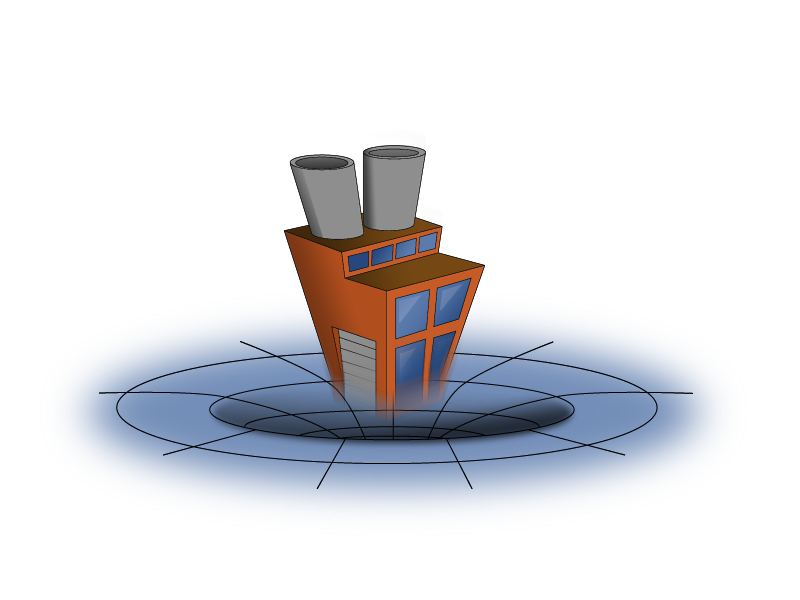
\includegraphics[height=0.6\textwidth]{factory}\\Simfactory\\\zhs{模拟工厂}\\
 \end{minipage}
 \begin{minipage}{0.3\textwidth}
  \centering
  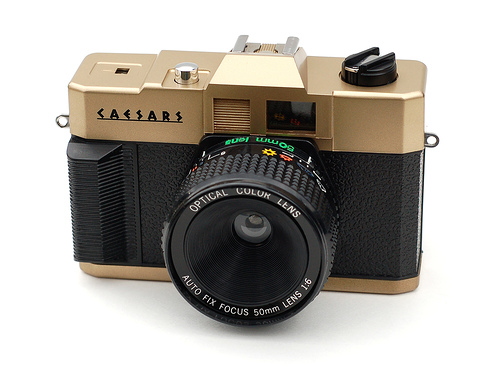
\includegraphics[height=0.6\textwidth]{camera}\\Formaline\\\zhs{福尔马林}\\
 \end{minipage}
}

\frame{\frametitle{Tools: GetComponents}
 \hspace{9cm}
\includegraphics[height=3cm]{cactuslogo}\\\vspace{-3cm}
 Task: Collect software from various repositories\\at different sites\\*[1em]
 Example simulation assembly:
 \begin{itemize}
  \item Cactus Flesh and Toolkit (svn.cactuscode.org)
  \item Core Einstein Toolkit (svn.einsteintoolkit.org)
  \item Carpet AMR (carpetcode.org, git)
  \item Tools, Parameter Files and Data (svn.einsteintoolkit.org)
  \item Group Modules (x.groupthorns.org)
  \item Individual Modules (x.mythorns.org)
 \end{itemize}
 x: cvs, svn, darcs, git, hg, http
}

\frame{\frametitle{Tools: Simulation Factory}
 \begin{centering}
  \small
  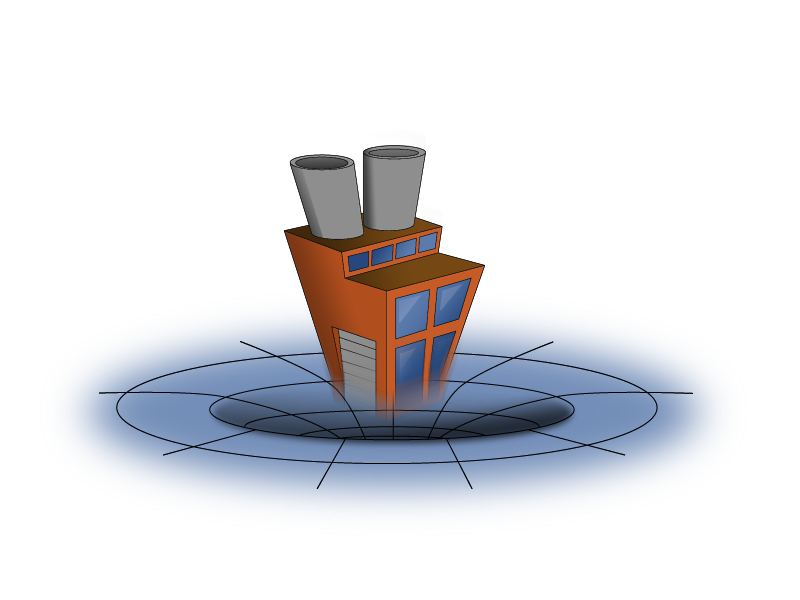
\includegraphics[height=3cm]{factory}\\
  \href{http://www.simfactory.org/}{http://www.simfactory.org/}\\
 \end{centering}\vspace{1em}
 Task: Provide support for common, repetitive steps:\\
 \begin{itemize}
  \item Access remote systems, synchronize source code trees
  \item Configure and build on different systems semi-automatically
  \item Provide maintained list of supercomputer configurations
  \item Manage simulations (follow ``best practices'', avoid human errors)
 \end{itemize}
}

\frame{\frametitle{Tools: Formaline}
 \hspace{8cm}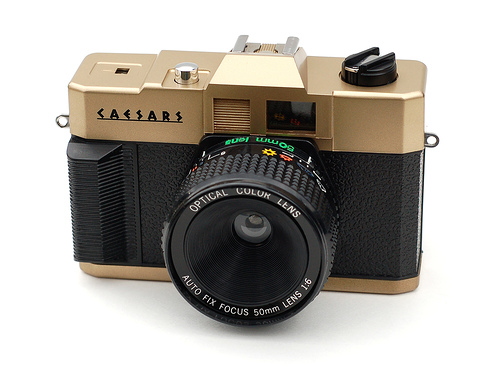
\includegraphics[height=2cm]{camera}\\
 \begin{itemize}
  \item Task: Ensure that simulations are and remain repeatable, remember
        exactly how they were performed
  \item Take snapshots of source code, system configuration; store it in
        executable and/or git repository
  \item Tag all output files
 \end{itemize}
}

\frame{\frametitle{CaFunwave}
 \begin{itemize}
  \item Based on Fenyan Shi's Funwave TVD code
  \item With bug fixes
  \item Identical to round-off double precision
  \item Supports various wavemakers
  \item Supports data from an input file
 \end{itemize}
}

\frame{\frametitle{CaFunwave}
 \begin{itemize}
  \item Paper with immersed boundary conditions
  \item Vegetation included, both integral and simple forms
  \item Can use AMR with fixed time step and dispersion turned off 
  \item Will use AMR with fixed time step and dispersion in the near future
 \end{itemize}
}

\end{document}

